%  /  significa lugares onde tem coisa para dar replace
%  ?? lugares onde estou em duvida.

Foram resolvidos dois tipos de acoplamento, o do Kinect ao servo motor e o do servo motor ao robô. O objetivo final desta solução era tornar a navegação autônoma mais confiável, pois em certas situações é necessário visualizar as laterais antes de rotacionar o robô. Por isso a necessidade de rotacionar o Kinect, possibilitando "olhar para os lados".

Para solucionar o problema de acoplamento entre o Kinect e o servo motor foram estudadas várias alternativas, entre elas a mais viável foi a encontrada em \cite{modelo3DMotorKinect}. Através do serviço de impressão 3D disponibilizado pelo Departamento Academico de Design Industrial (DADIN) foi possível produzir a peça de acoplamento de forma rápida e barata. O material utilizado na impressão foi o Acrilonitrila Butadieno Estireno (ABS), muito usado para este tipo de serviço. A Figura \ref{fig:modeloMotorKinect} apresenta o modelo no computador e o impresso.

\begin{figure}[H]
\centering
\begin{tabular}{cc}
  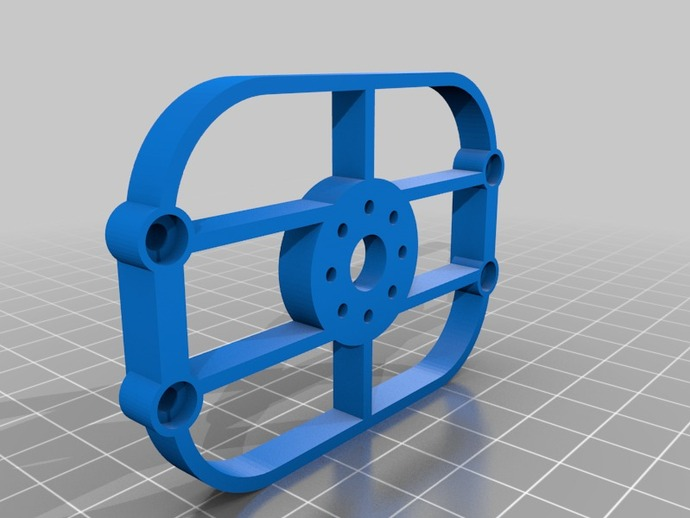
\includegraphics[width=4cm, height=3cm]{images/modeloMotorKinect.jpg} &
  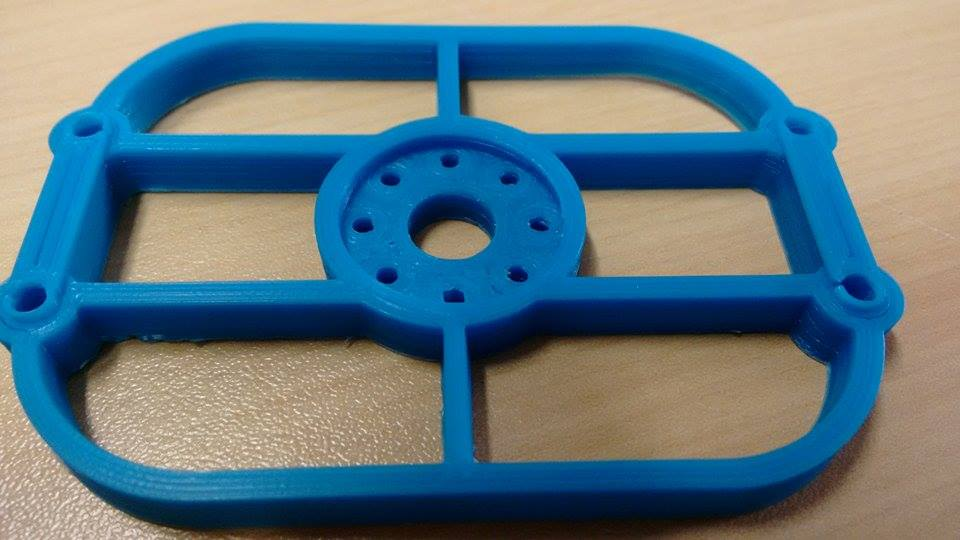
\includegraphics[width=4cm, height=3cm]{images/acoplamentoMotor.jpg} \\
 (a) & (b)
\end{tabular} 
\caption{\small{(a) Modelo sugerido por ~\cite{modelo3DMotorKinect} para acoplar o motor ao Kinect. (b) Peça impressa no DADIN.}}
\label{fig:modeloMotorKinect}
\end{figure} 

O problema de fixação do motor ao robô deveria ser solucionado de forma não invasiva, ou seja, sem alterar a estrutura do robô ou do motor. O projeto para esta peça foi feito no \textit{SketchUp Make 2015}. A Figura \ref{fig:modeloCimaMotorKinect} mostra a peça projetada e a Figura \ref{fig:kinectMontado} apresenta a estrutura final com o Kinect acoplado. Foi escolhida madeira como material para fixar o motor ao robo pois ela é de fácil acesso e manuseio, assim possibilitando o ajuste do modelo durante o projeto.

\begin{figure}[H]
\centering
  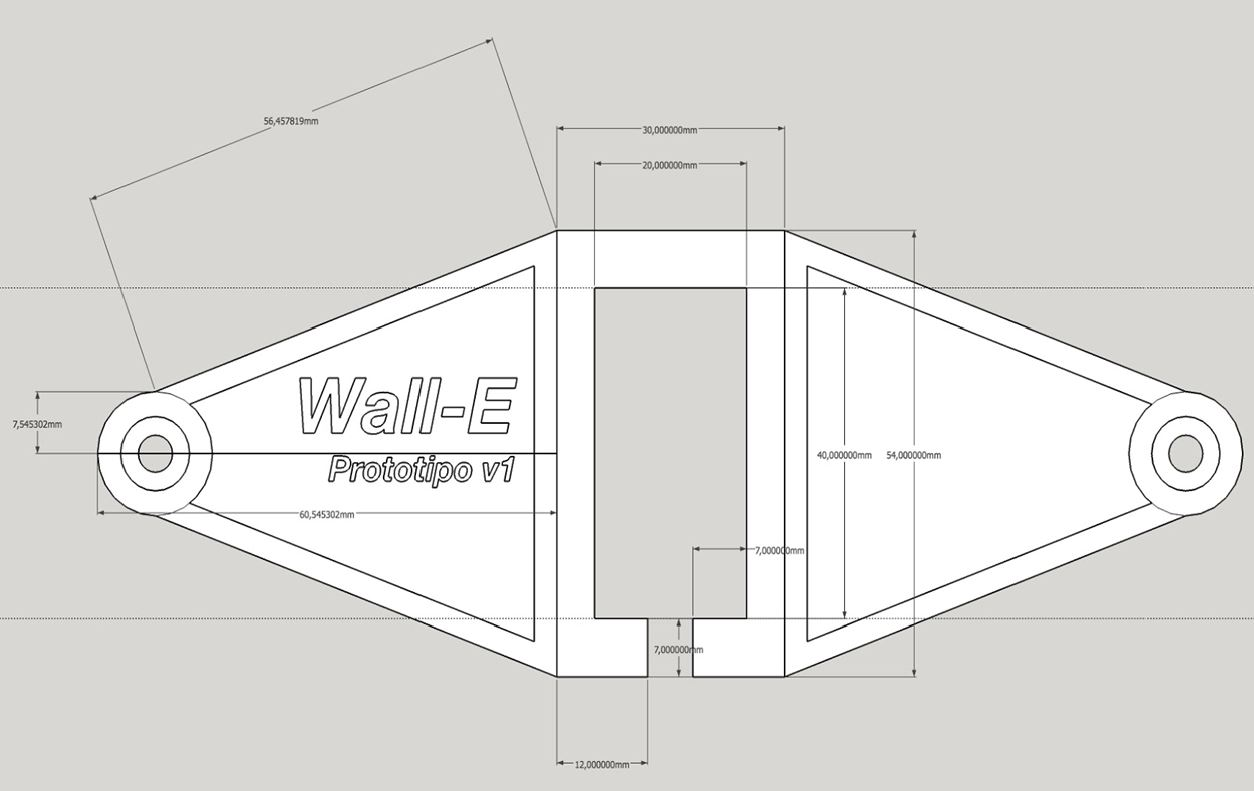
\includegraphics[scale=.35]{images/visaoCimaMotorKinect.jpg} 
\caption{\small{Modelo feito no \textit{SketchUp Make 2015} para acoplar o motor ao robô.}}
\label{fig:modeloCimaMotorKinect}
\end{figure} 

